\maketitle
\tableofcontents
\newpage

\section{Zielsetzung}
Gegenstand des Versuches ist der Lock-In-Verstärker, dessen Funktionsweise
erforscht werden soll.
\section{Theorie}
Der Lock-In-Verstärker wird überwiegend bei Messungen mit stark verrauschten Signalen
verwendet, um die gesuchte Frequenz herauszufiltern, ähnlich wie mit einem Bandpass.
Die Güte des Lock-In-Verstärkers liegt allerdings etwa um den Faktor 100 höher als
der eines Bandpasses.
\begin{equation}
    U_{out} = \frac{2}{\pi} \, U_0
    \label{eqn:4}
\end{equation}
Mit einer Phasendifferenz $\phi$ zwischen Signal- und Referenzspannung wird
\eqref{eqn:4} zu
\begin{equation}
  U_{out} = \frac{2}{\pi} \, U_0 \, \symup{cos}(\phi)
  \label{eqn:5}
\end{equation}
\section{Durchführung}
\subsection{Versuchsaufbau}

\section{Fehlerrechnung}
Es gibt:
\begin{equation}
  \bar{T} = \frac{1}{n} \sum_{i=1}^{n} T_{i}
  \label{eqn:1}
\end{equation}
den Mittelwert und:
\begin{equation}
  \sigma_{\bar{T}} = \sqrt{\frac{1}{n(n-1)} \sum_{i=1}^{n}(\bar{T}-T_i)^2}
  \label{eqn:2}
\end{equation}
den Fehler des Mittelwertes. Falls zwei fehlerbehaftete Größen in einer Gleichung
zur Bestimmung einer anderen Größe Verwendung finden, dann berechnte sich der Gesamtfehler
nach der Gaußschen Fehlerfortpflanzung zu
\begin{equation}
    \symup \Delta f(x_1, x_2, ..., x_n) = \sqrt{\left(\frac{\symup df}{\symup dx_1} \symup \Delta
    x_1 \right)^2 +    \left(\frac{\symup df}{\symup dx_2} \symup \Delta
    x_2 \right)^2 + ... + \left(\frac{\symup df}{\symup dx_n} \symup \Delta x_n \right)^2} \ .
    \label{eqn:3}
\end{equation}

\section{Auswertung}
\subsection{Verwendung des Lock-In Verstärkers mit und ohne künstlichem Rauschen}
\begin{table}
  \centering
  \caption{Mit Gain von 5 gemessene Werte}
  \label{tab:1}
  \begin{tabular}{c c c}
    \toprule
    Phase/$\si{\pi}$ & $U_{unverauscht}/\si{\volt}$ & $U_{verauscht}/\si{\volt}$ \\
    \midrule
    0.00 & 6.00 & 6.00 \\
    0.17 & 5.00 & 5.00 \\
    0.25 & 3.50 & 3.50 \\
    0.33 & 1.50 & 1.50 \\
    0.50 & -1.00 & -1.00 \\
    0.67 & -3.50 & -3.50 \\
    0.75 & -5.00 & -5.00 \\
    0.83 & -6.00 & -6.00 \\
    1.00 & -6.00 & -6.00 \\
    1.25 & -3.50 & -3.50 \\
    1.50 & 1.00 & 1.00 \\
    1.83 & 6.00 & 6.00 \\
    \bottomrule
  \end{tabular}
\end{table}
\begin{figure}
  \centering
     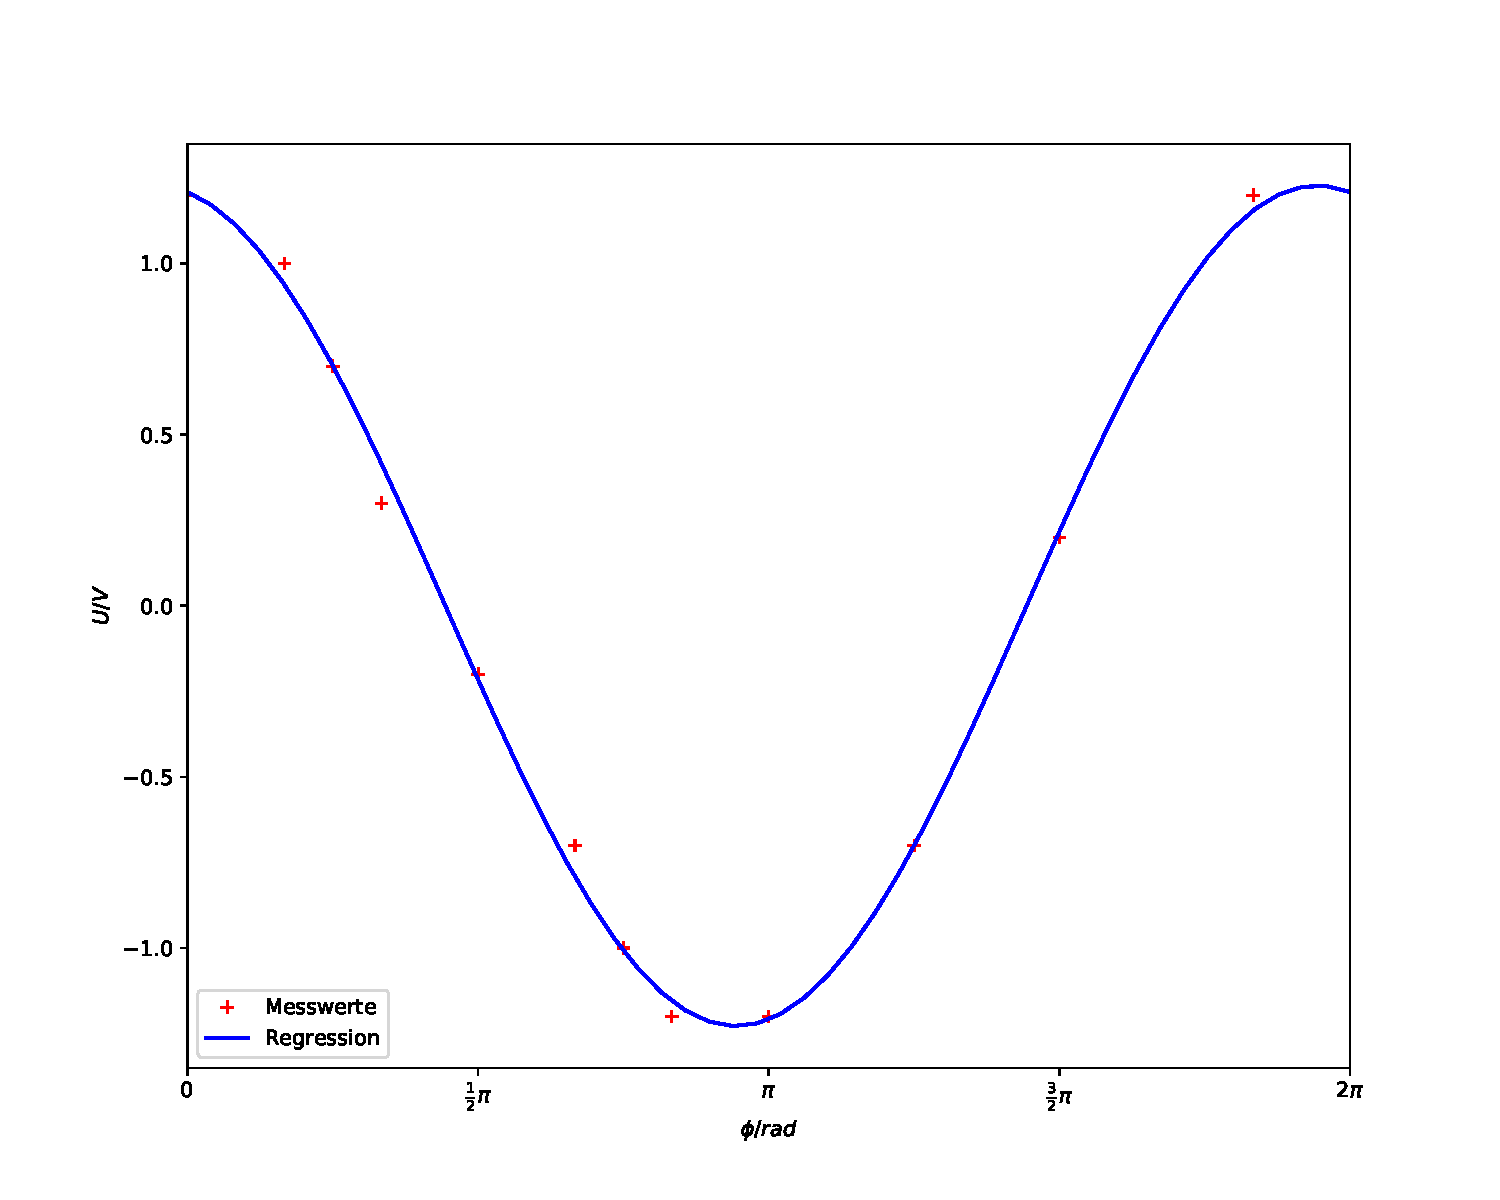
\includegraphics[scale=0.6]{UvonPhi.pdf}
  \caption{Auftragen der gemessenen Spannungen gegen die Phasen mit Regression. Die Spannungen sind vom Verstärkungsfaktor bereinigt.}
  \label{plot:1}
\end{figure}
Die am Tiefpassfilter mit und ohne Rauschen gemessenen Spannungen sind in Tabelle \ref{tab:1}
dargestellt. Es zeigt sich kein messbarer Unterschied zwischen unverrauschter und verrauschter Messung,
woraus auf die Ordnungsgemäße Funktionsweise des Aufbaus geschlossen werden kann.
Die Messwerte wurden bei einem Verstärkungsfaktor von 5 gemessen. Wird die Phase gegen die Spannung
aufgetragen, ergibt sich der in Grafik \ref{plot:1} dargestellte Verlauf. Werden die Messwerte mit einer
Funktion:
\begin{equation*}
  U_{out}(\phi) = A_0 \cdot \symup{cos}(\phi + \symup{\delta}\phi)
\end{equation*}
gefittet, wobei $A_0$ die Amplitude und $\symup{\delta}\phi$ die interne Phase des Aufbaus darstellt,
ergeben sich folgende Werte für Amplitude und Phase:
\begin{equation*}
  \begin{split}
    A_0 = \SI{1.228(22)}{\volt} \\
    \symup{\delta}\phi = \SI{0.177(19)}{\pi}
  \end{split}
\end{equation*}
Die gemessenen Werte folgen also dem nach \eqref{eqn:5} zu erwartenen Verlauf.

\section{Diskussion}
\newpage
\nocite{*}
\printbibliography
